\documentclass[algebra]{subfiles}

\begin{document}
    \section{Характеристический многочлен матрицы и оператора. Независимость характеристического многочлена оператора от выбора базиса.}
        \begin{Definition}
          \[A \in M_n(K)\]
          Характеристический многочлен A
          \[\det (A - tE) = \mathcal{X}_A(t)\]

          \[\begin{vmatrix}
            &a_{11} - t & a_{12} & ... & a_{1n}&\\
            &a_{21}     & \ddots&\\
            &\vdots     &        & \ddots&\\
            &a_{n1}    &         &     & a_{nn} - t &
          \end{vmatrix}
          = (-1)^n t^n + (-1)^{n - 1} (a_{11} + ... + a_{nn}) t^{n - 1} + ... + \det A
          \]

          \[V \text{ - в.п.} \q \dim V = n < \infty \q v_1, ..., v_n \text{ - базис } V\]
          \[f \in \End \ (V) \q A = [f]_{\{v_i\}}  \text{ - матрица оператора в базисе } v_1, ..., v_n \]
          \[\mathcal{X}_f(t) = \mathcal{X}_A(t)\]
        \end{Definition}

        \begin{lemma}
          Характеристический многочлен f не зависит от выбора базиса в V
        \end{lemma}

        \begin{Proof}
            \[\begin{matrix}
                v_1, ..., v_n\\
              v_1', ..., v'_n
            \end{matrix} \text{ - базисы } V \q\q \begin{matrix}
          C &\text{ - матрица преобр. координат }\\
            &\text{при переходе от } \{v_i\} к \{v_i'\}
            \end{matrix}\]
          \[A = [f]_{\{v_i\}} \]
          \[A' = [f]_{\{v_i'\}} \]
          \[A' = C'AC \q (A \text{ и } A' \text{ сократимы при помощи } C)\]
          \[? \mathcal{X}_{A'}(t) = \mathcal{X}_A(t) \]
          \[\mathcal{X}_{A'}(t) = \det(C^{-1}AC - tE)  = \det (C^{-1}AC - C^{-1}(tE)C) = \]
          \[ = \det(C^{-1}(A - tE)C) = \det(C^{-1}) \cdot \det(A - tE) \cdot \det(C) = \]
          \[= \det(A - tE) = \mathcal{X}_A(t)\]
        \end{Proof}


    \section{Собственные числа и собственные векторы оператора и матрицы.
      Собственные числа как корни характеристического многочлена}

      \begin{Definition}
        \[f \in \End(V) \q \lambda \in K\]
        \[\lambda \text{ - собственное число } f, \text{ если } \exists v \neq 0; \q v \in V : f(v) =
        \lambda \cdot v\]
        \[\text{Если } \lambda \text{ - собс. число } f \q v \in  V \q f(v) = \lambda v \text{, то } v
        \text{ - собс вектор}\]
      \end{Definition}

      \begin{Definition}
        \[\lambda \text{ - с.ч. } f \Ra V_\lambda = \{v : f(v) = \lambda v\}\]
        Поэтому удобно 0 считать с.в.
      \end{Definition}

      \begin{Definition}
        \[A \in M_n(K)\]
        \[\lambda \text{ - с.ч } A \text{, если } \exists v \neq \begin{pmatrix}
          0\\
          \vdots\\
          0
        \end{pmatrix} \in K^n : A_n = \lambda_n\]
      \end{Definition}

      \begin{Theorem}
        \[A \in M_n(K)\]
        \[\lambda \in  K \text{ - с.ч. }A \rla \lambda  \text{ - корень } \mathcal{X}_A(t)\]
      \end{Theorem}

      \begin{Proof}
          \[\exists v \neq 0 \q Av = \lambda v\]
        \[\Br{A - \lambda E} v = 0\]
        Рассмотрим коэф. столбца V как неизвестные
        \[\lambda \text{ - с.ч. }A \rla (A - \lambda E)v = 0 \text{ - имеет нетривиальный ранг} \]
        \[\rla \det(A - \lambda E) = 0 \rla \mathcal{X}_A(\lambda) = 0 \rla \lambda \text{ - корень }
        \mathcal{X}_A(t)\]
      \end{Proof}

      \begin{Consequence}
        \[\dim V = n < \infty \q f \in \End(V)\]
        \[\lambda \in K \text{ - с.ч. } f \rla \lambda \text{ - корень } \mathcal{X}_f(t)\]
      \end{Consequence}

      \begin{Proof}
          \[\text{Фиксируем базис } v_1, ..., v_n\]
        \[f \ra [f] = A \q\q v \ra \begin{pmatrix}
          a_1\\
          \vdots\\
          a_n
        \end{pmatrix} = [v]\]
        \[\rla v \text{ - с.в. } f \text{, отвеч. } \lambda \q\q \begin{pmatrix}
          a_1\\
          \vdots\\
          a_n
        \end{pmatrix} \text{ - с.в. } A \text{, отвеч. } A\]
      \end{Proof}


    \section{Теорема Гамильтона-Кэли.}
        \begin{Theorem}
          \[A \in M_n(K) \q \mathcal{X}_A(A) = 0_{M_{n}(K) } \]
        \end{Theorem}

        \begin{proof}
          \begin{figure}[H]
                  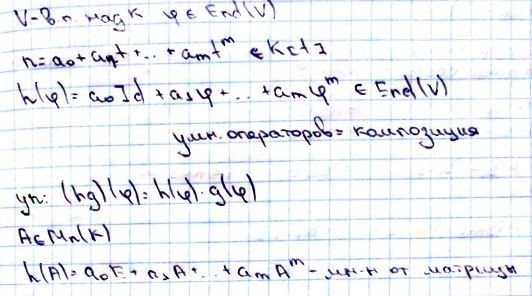
\includegraphics[width=10cm]{pics/53_1}
                  \centering
          \end{figure}
        \end{proof}

        \begin{consequence}
          \begin{figure}[H]
                  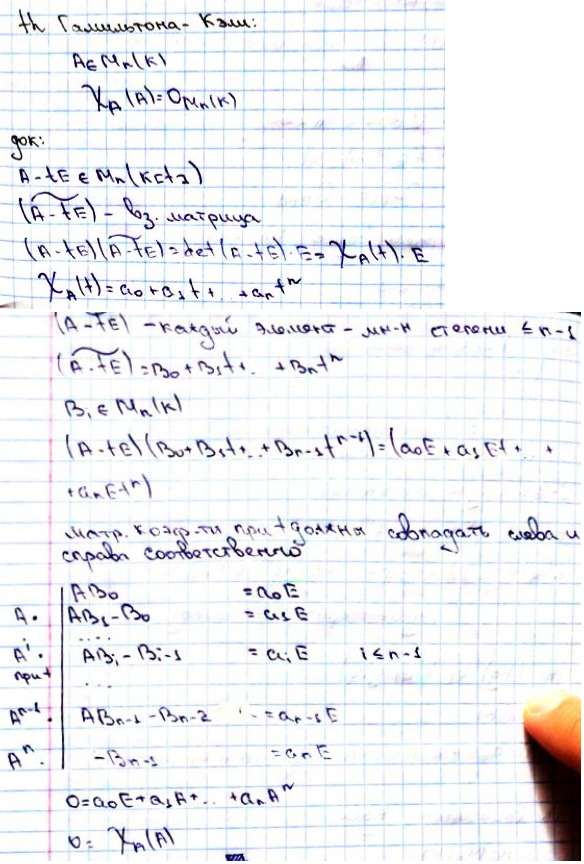
\includegraphics[width=10cm]{pics/53_2}
                  \centering
          \end{figure}
        \end{consequence}

        \begin{proof}
          \begin{figure}[H]
                  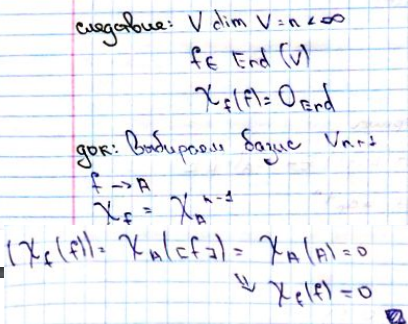
\includegraphics[width=10cm]{pics/53_3}
                  \centering
          \end{figure}
        \end{proof}


    \section{Диагонализируемые операторы. Критерий диагонализируемости. Примеры недиагонализируемых операторов}
        \begin{Definition}
            \[V \text{ - в.п. над } K \q \dim V = n < \infty\]
          \[\varphi \in \End(V)\]
          \[\varphi \text{ - диагонализируем, если } \exists \text{ базис } V, \text{ в котором матрица }
          \varphi \text{ - диагональна}\]
        \end{Definition}

        \begin{Theorem}
            \[V \text{ - в.п. } \q \dim V = n < \infty\]
            \[\varphi \in \End(V)\]
            \[\varphi \text{ - диагонализируем } \rla \exists \text{ базис } V \text{, состоящий из собс.
            векторов }\varphi\]
        \end{Theorem}

        \begin{Proof}
            \[\Ra v_1, ..., v_n \text{ - базис}\]
          \[[\varphi] _{\{v_i\}} = \begin{pmatrix}
            \lambda_1 &        & 0\\
                      & \ddots    \\
            0         &        & \lambda_n
          \end{pmatrix} \]
          \[\varphi(v_i) = \lambda_i v_i \q v_i \neq 0 \Ra v_i \text{ - с.в.}\]
          \[\La v_1, ..., v_m \text{ - базис из с. в. } \varphi\]
          \[\varphi(v_i) = \lambda_i v_i \q \lambda \in K\]
          \[\varphi(v_i) = 0 \cdot v_1 + ... + 0 \cdot v_{i - 1} + \lambda_i v_i +
          0 \cdot v_{i + 1} + ... \]
          \[[\varphi]_{\{v_i\}} = \begin{pmatrix}
            \lambda_1 & 	  & 0\\
                  &\ddots &\\
            0 		  & 	  & \lambda_n
          \end{pmatrix} \]
        \end{Proof}

        \begin{Example}
            \[V = \CC^2\]
            \[\varphi(x) = A \cdot x \q\q A = \begin{pmatrix}
              0 & 1\\
              0 & 0
            \end{pmatrix}\]
            \[\mathcal{X}_{\varphi}(t) = \mathcal{X}_A(t) = t^2 \q \text{ c.ч } \lambda = 0 \]
            \[Ax = 0\]
            \[\rk A = 1 \q \text{2 перем } \Ra \text{ пр-во решений одномерно}\]
            $\Ra$ все с.в. лежат в одномерном пр-ве $\Ra$ непорожд $\CC^2$ \\
            $\Ra$ не диагонализ.
        \end{Example}

        \begin{Example}
          \[V = K[x]_n = \{f \in K[x];\  \deg f \leq n\}\]
          \[\Char K = 0\]
          \[\varphi = \frac{\partial }{\partial x} \q\q \varphi(f) = f'\]
          \[\text{с.ч. } \lambda = 0\]
          \[\text{с.в. пр. : константы}\]
          \[\dim V = n + 1 \q (n \geq 1 \Ra \varphi \text{ - не диагонализ})\]
        \end{Example}


    \section{Инвариантные подпространства. Матрице линейного оператора, действующего на пространстве, разложенном в прямую сумму инвариантных подпространств.}
    *здесь когда-нибудь будет что-то*
    \begin{examples}
      *здесь когда-нибудь будут примеры*
    \end{examples}

    \begin{theorem}[1]
      *здесь когда-нибудь будет теорема*
    \end{theorem}

    \begin{proof}
      *здесь когда-нибудь будет док-во*
    \end{proof}

    \begin{theorem}[2]
      *здесь когда-нибудь будет теорема*
    \end{theorem}

    \begin{proof}
      *здесь когда-нибудь будет док-во*
    \end{proof}

    \begin{figure}[H]
            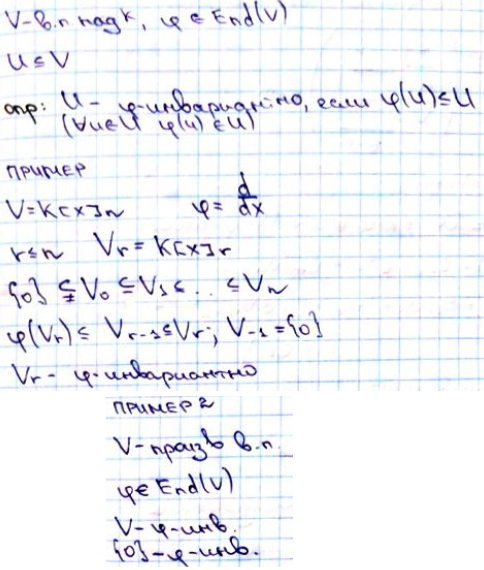
\includegraphics[width=10cm]{pics/55_1}
            \centering
    \end{figure}
    \begin{figure}[H]
            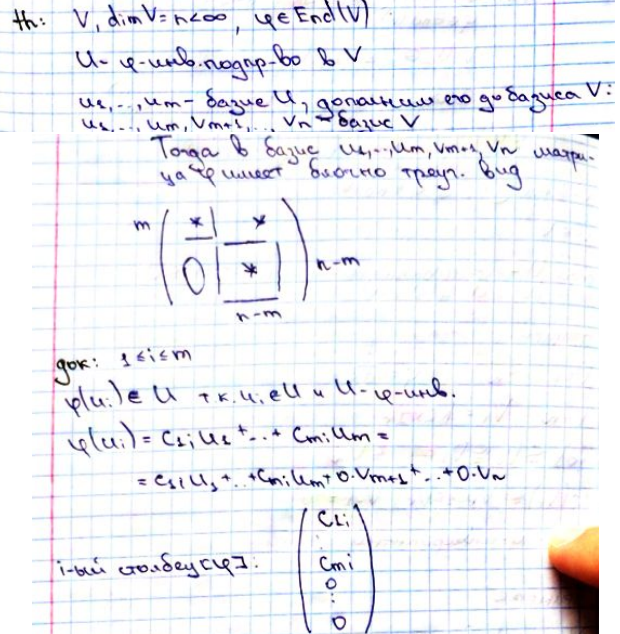
\includegraphics[width=10cm]{pics/55_2}
            \centering
    \end{figure}
    \begin{figure}[H]
            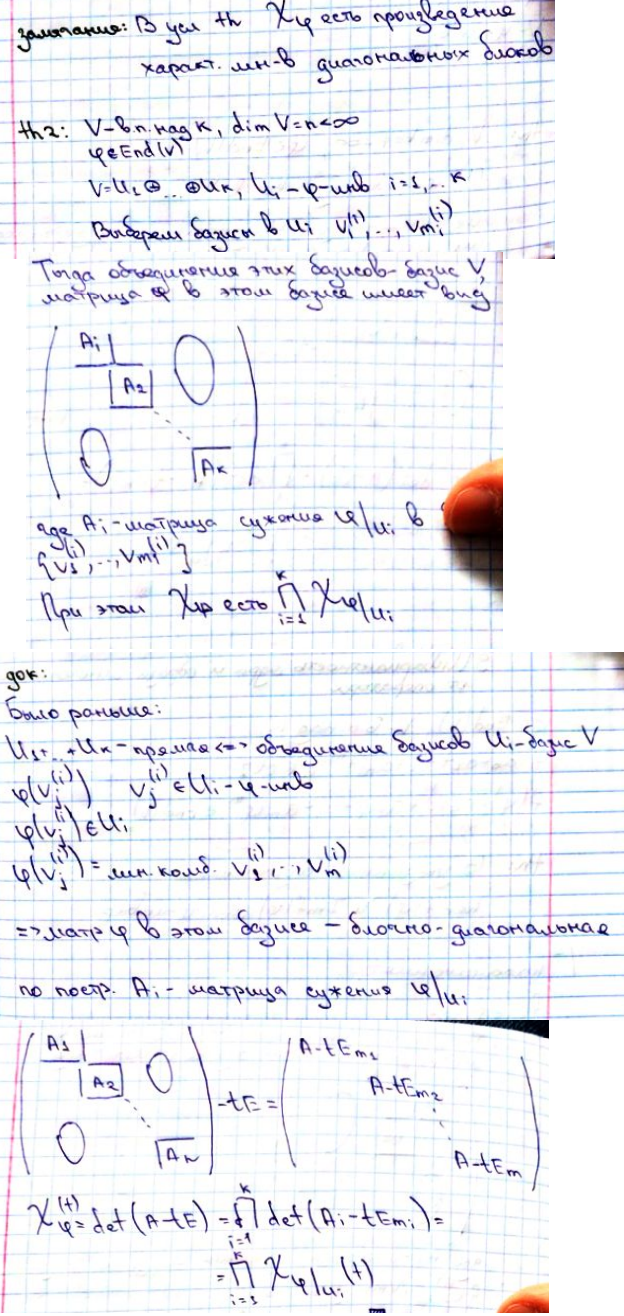
\includegraphics[width=10cm]{pics/55_3}
            \centering
    \end{figure}

    \section{Инвариантность ядра и образа многочлена от оператора.}
    *здесь когда-нибудь будет что-то*
    \begin{theorem}
      *здесь когда-нибудь будет теорема*
    \end{theorem}

    \begin{proof}
      *здесь когда-нибудь будет док-во*
    \end{proof}

    \begin{figure}[H]
            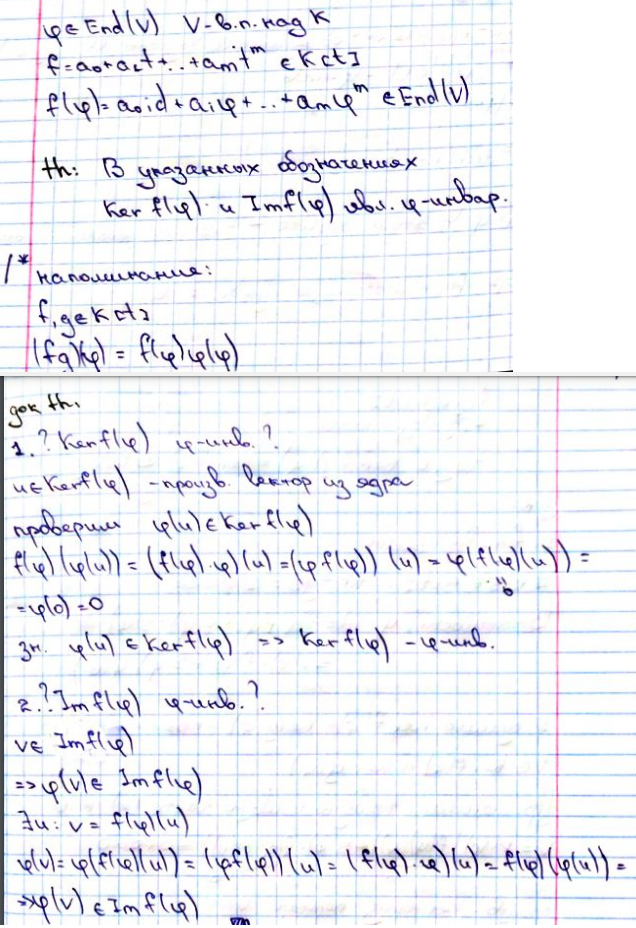
\includegraphics[width=10cm]{pics/56}
            \centering
    \end{figure}

    \section{Теорема о разложении $\Ker(f g)(\phi)$ в прямую сумму инвариантных подпространств и следствия из неё.}

    \begin{theorem}
      *здесь когда-нибудь будет теорема*
    \end{theorem}

    \begin{proof}
      *здесь когда-нибудь будет док-во*
    \end{proof}

    \begin{figure}[H]
            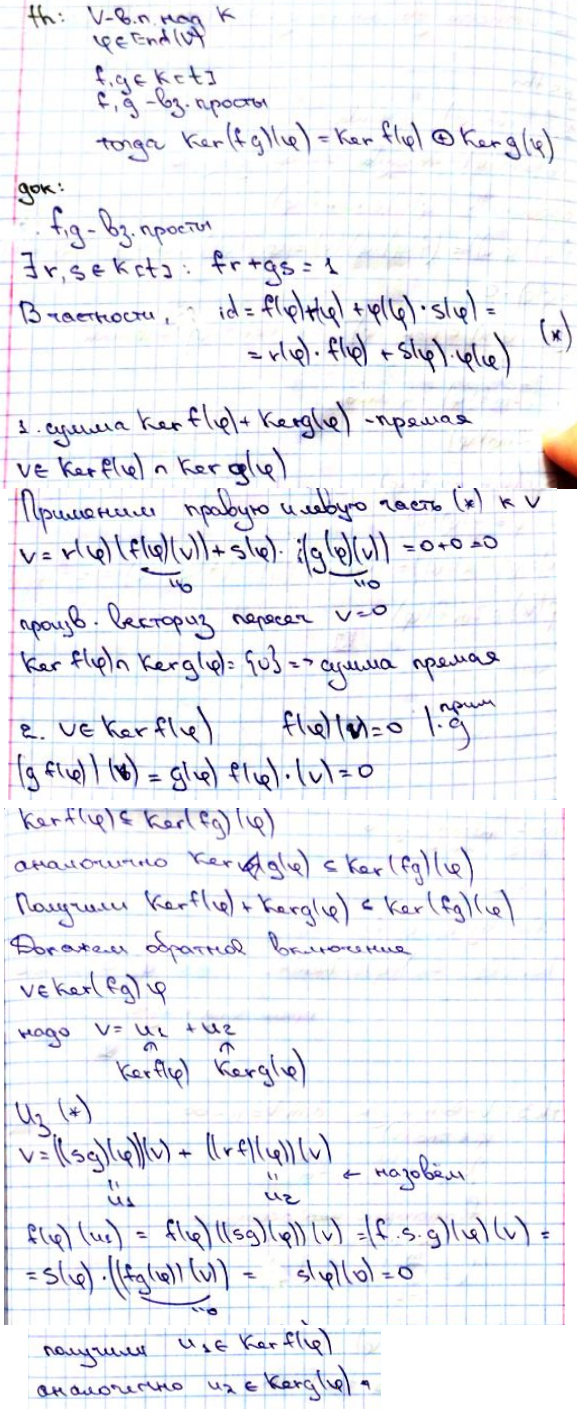
\includegraphics[width=10cm]{pics/57_1}
            \centering
    \end{figure}
    \begin{figure}[H]
            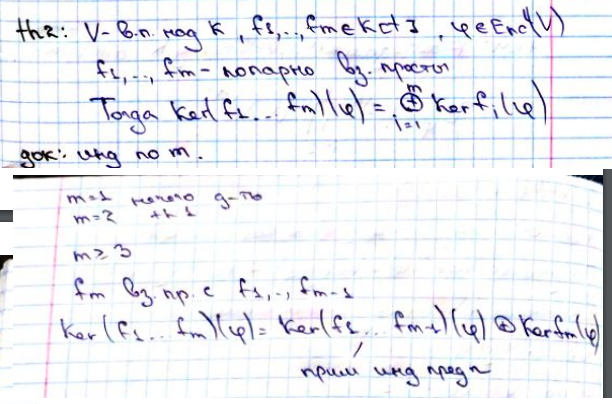
\includegraphics[width=10cm]{pics/57_2}
            \centering
    \end{figure}
    \begin{figure}[H]
            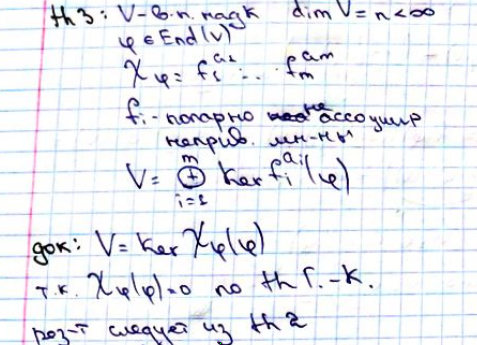
\includegraphics[width=10cm]{pics/57_3}
            \centering
    \end{figure}
    \begin{figure}[H]
            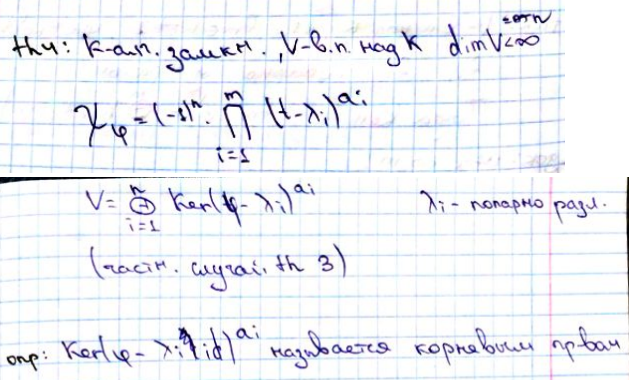
\includegraphics[width=10cm]{pics/57_4}
            \centering
    \end{figure}

    \section{Жорданова форма оператора. Жорданов базис. Формулировка теоремы о жордановой форме оператора. Сведение к случаю оператора с единственным собственным числом.}
      \begin{Definition}
          \[\lambda \in K\]
          \[\mathfrak{J}(\lambda) = \begin{pmatrix}
            \lambda & & & 0\\
            1       & \ddots &\\
                    & \ddots & \ddots\\
            0 & & 1 &\lambda
          \end{pmatrix} \text{- жордан. клетка размера } n \text{ отвечающей }\lambda \]
          \[A \text{ - жорд. матрица, если }A \text{ - блочно диаг, а диг. блоки - жорд. клетки}\]
          \[\mathfrak{J}_1 = (\lambda)\]
          \[\mathfrak{J}_2 = \begin{pmatrix}
            \lambda & 0\\
            0       & \lambda
          \end{pmatrix}\]
          \[A = \begin{pmatrix}
            \mathfrak{J}_{m1}(\lambda_1) & & & 0\\
            & \mathfrak{J}_{m2}(\lambda_2)\\
            & &  \ddots &\\
            0 & & & \mathfrak{J}_{mk}(\lambda_k)
          \end{pmatrix}\]
      \end{Definition}

      \begin{Theorem} [1]
          \[K \text{ - алг. замк.} \q V, \q \dim V = n  < \infty\]
          \[\varphi \in \End(V)\]
          Тогда  $\exists$ базис пр-ва V,  в котором матрица $ \varphi$
          является жордановой матрицей.
          Причем клетки опред. однозначно с точностью до перестановки диаг. блоков\\
          *здесь когда-нибудь это будет дописано*
      \end{Theorem}

      \begin{consequence}
        *здесь когда-нибудь будет замечание*
      \end{consequence}

      \begin{theorem}[1']
        *здесь когда-нибудь будет теорема*
      \end{theorem}

      \begin{figure}[H]
              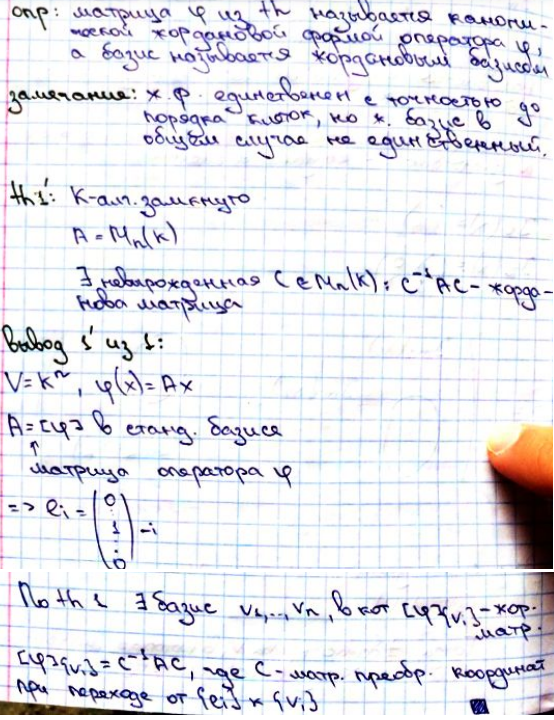
\includegraphics[width=10cm]{pics/58}
              \centering
      \end{figure}

    \section{Относительная линейная независимость. Относительные базисы. Корневые пространства. Лемма о спуске для корневых подпространств.}

    *здесь когда-нибудь будет что-то*

    \begin{lemma}[1]
      *здесь когда-нибудь будет лемма*
    \end{lemma}

    *здесь когда-нибудь будет вывод*

    *здесь когда-нибудь будет что-то*
    \begin{figure}[H]
            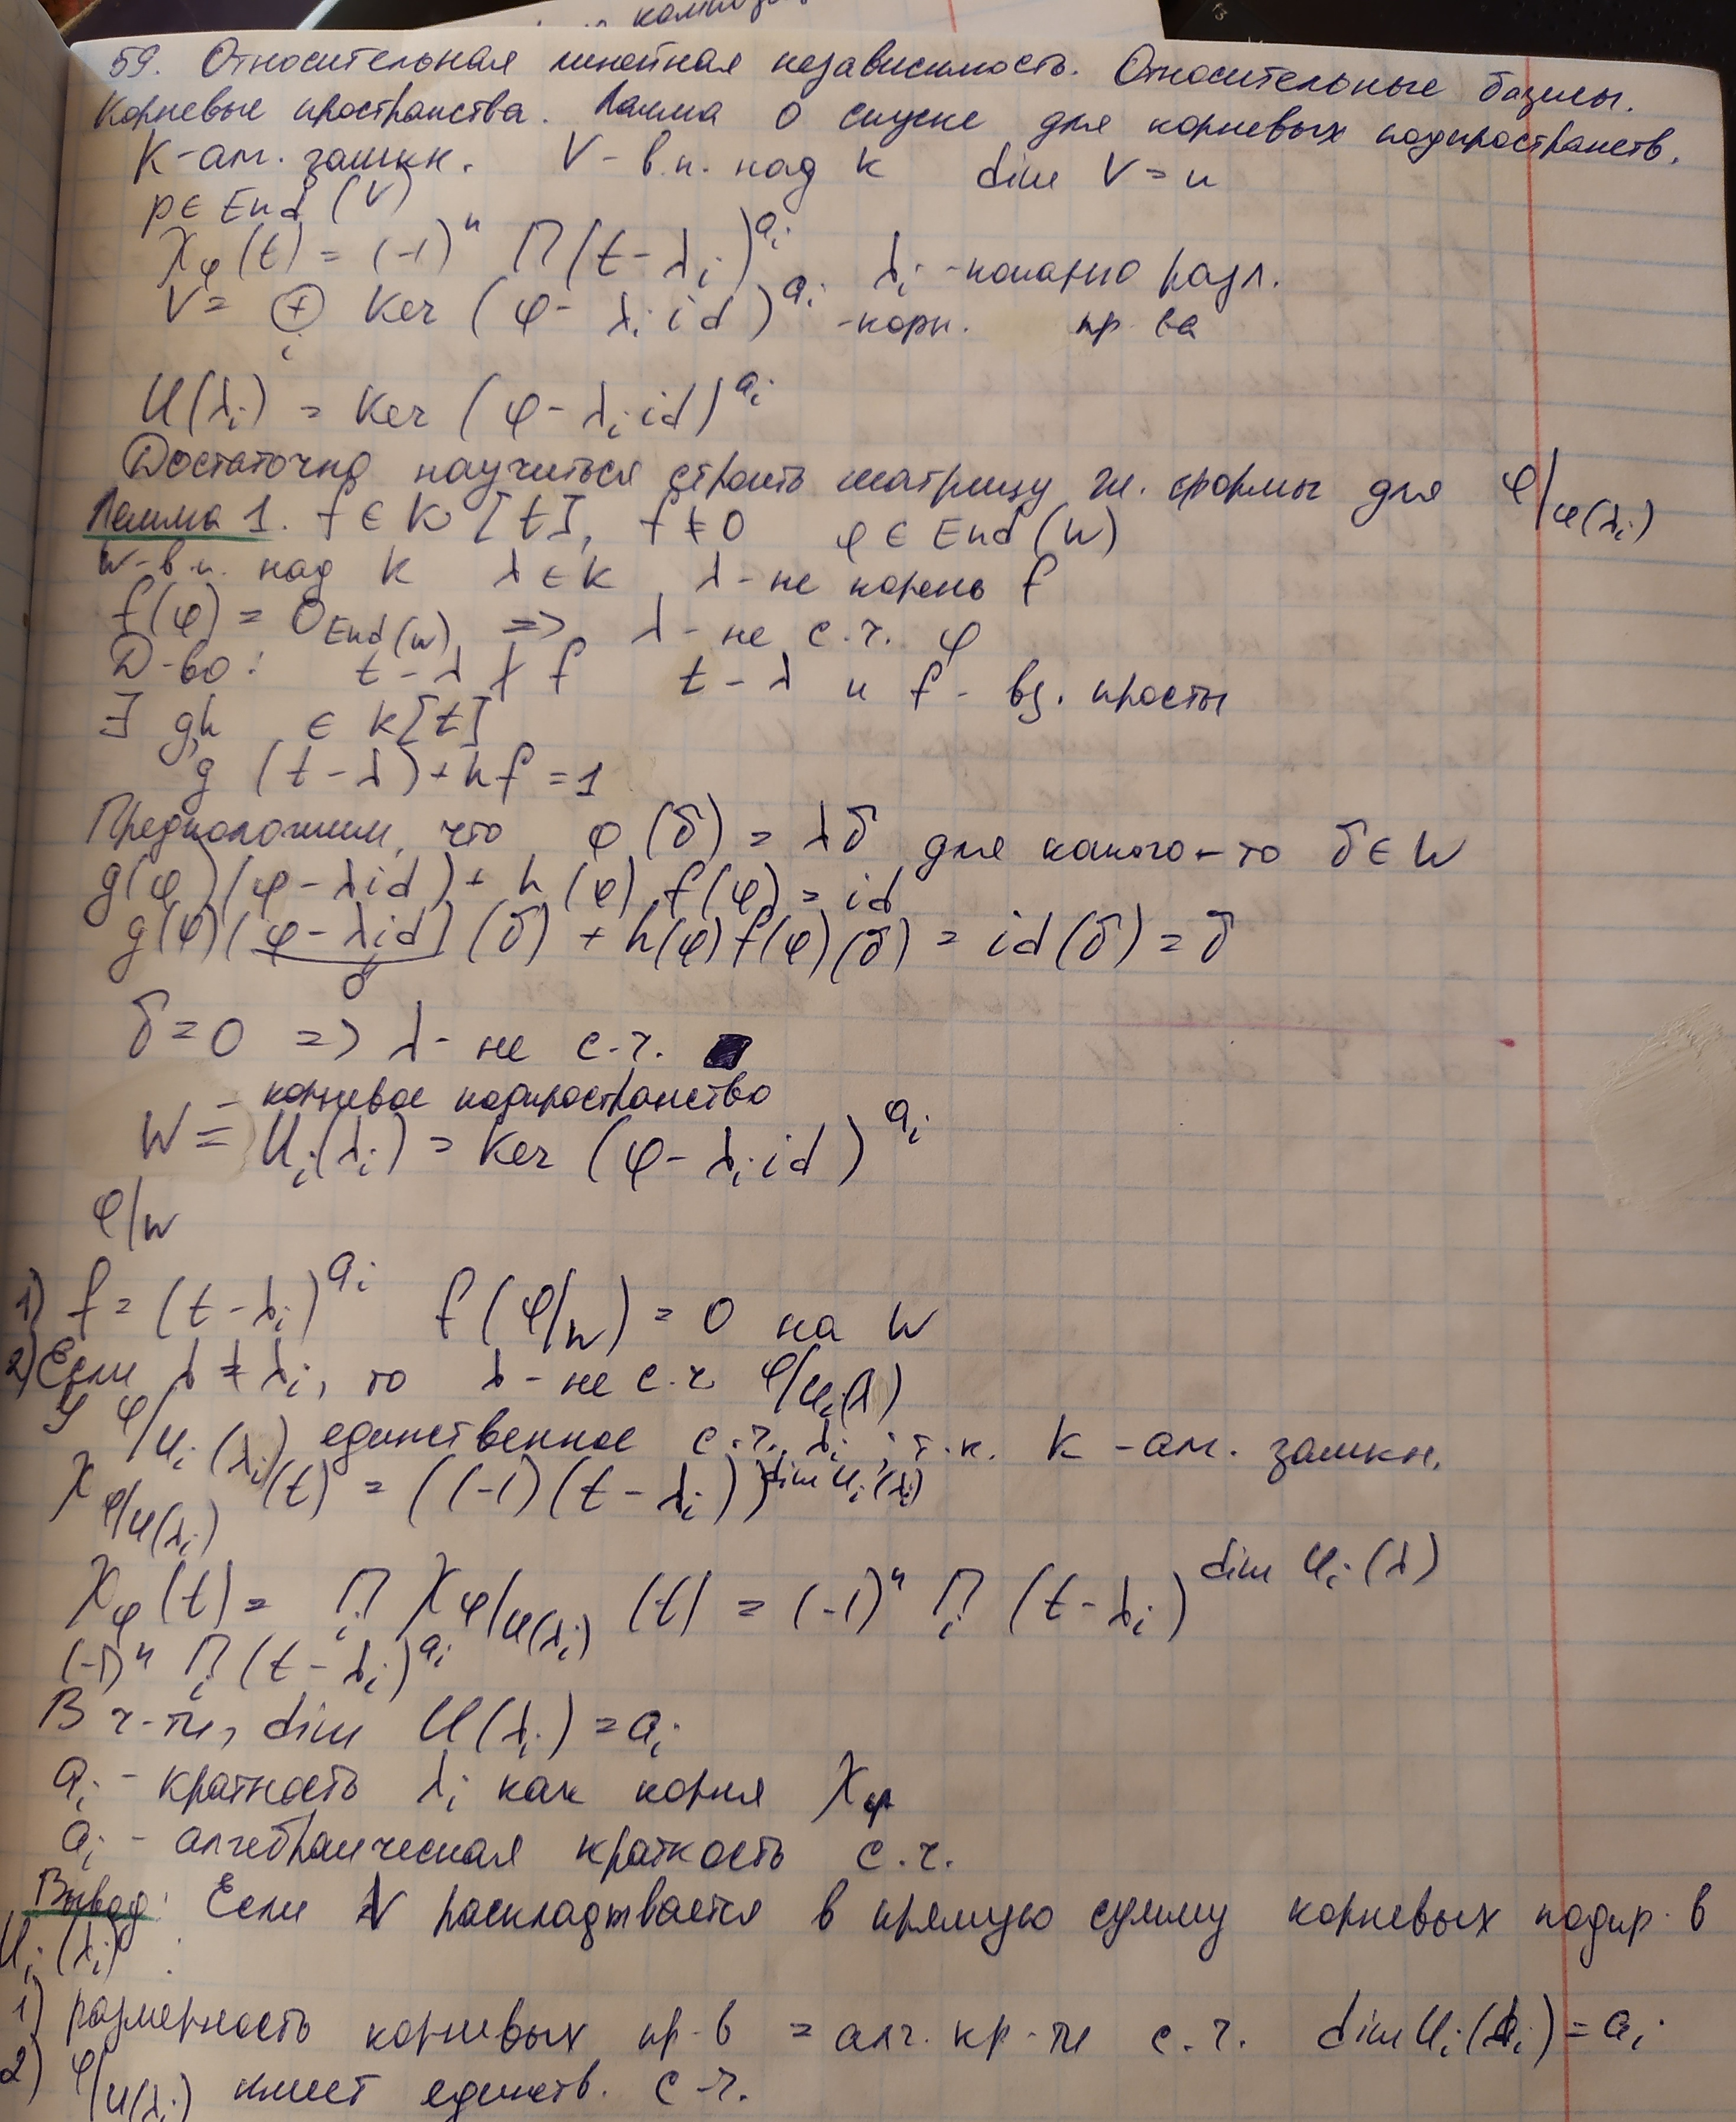
\includegraphics[width=10cm]{pics/l59_1}
            \centering
    \end{figure}
    \begin{figure}[H]
            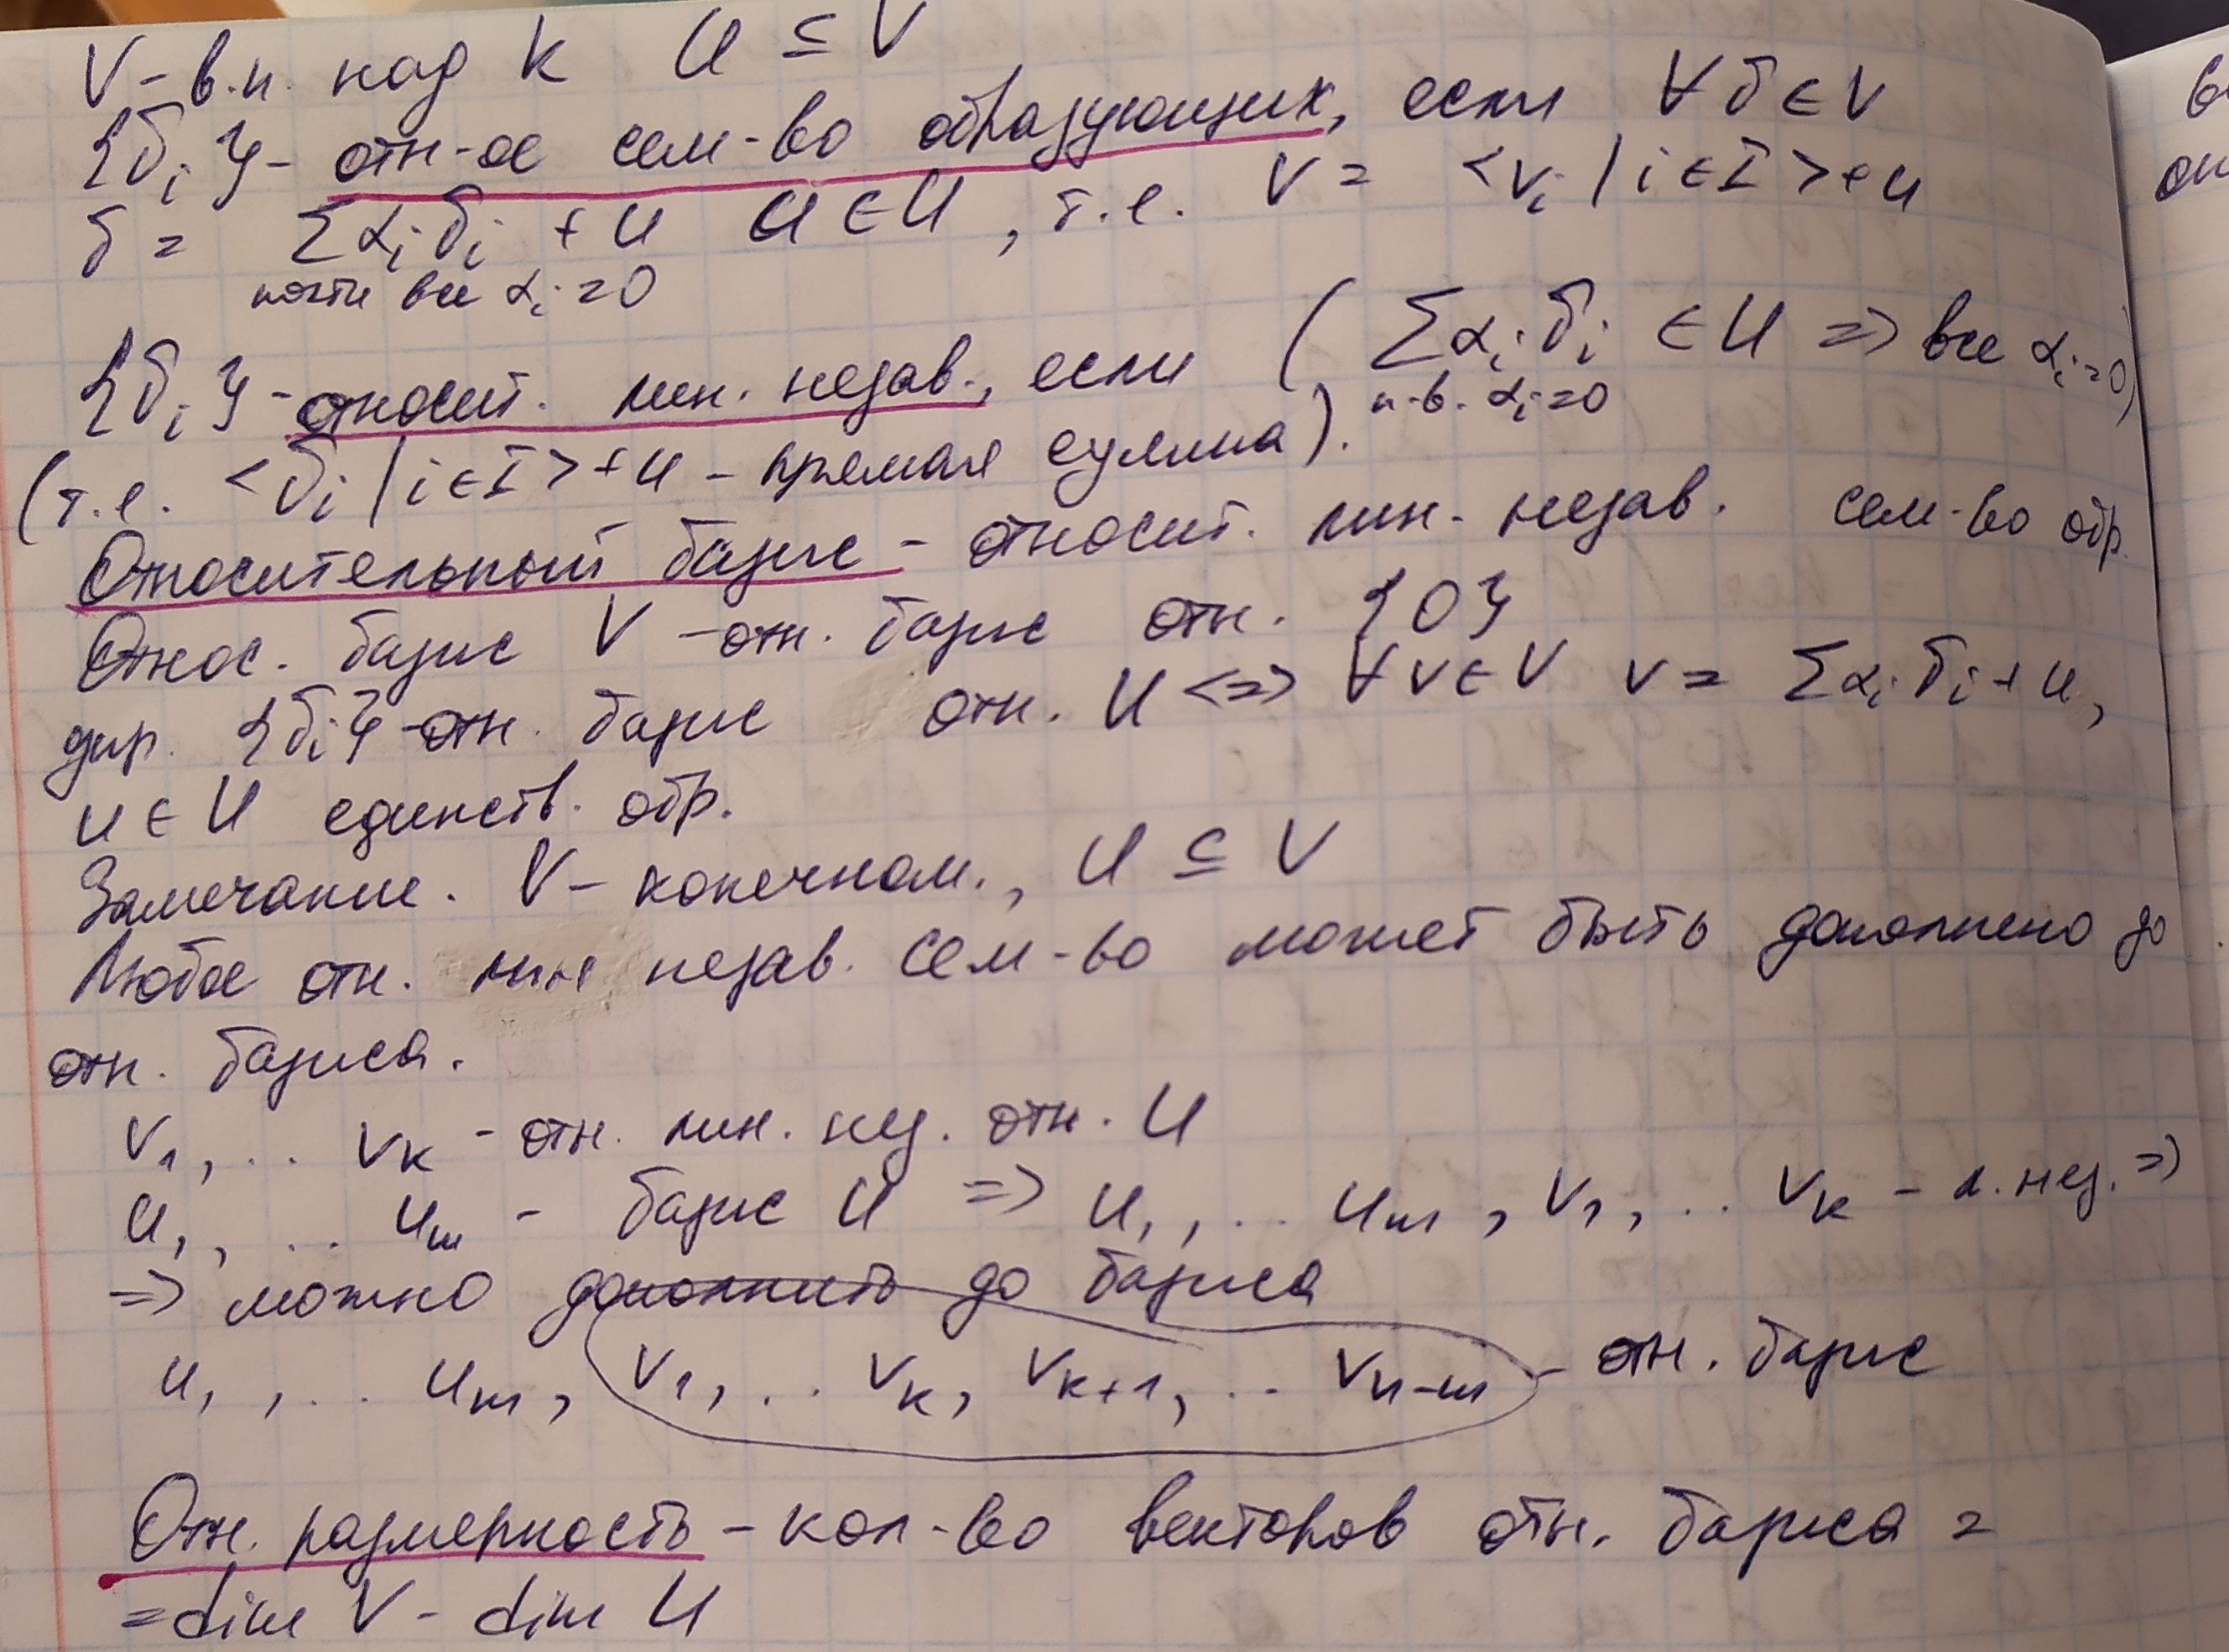
\includegraphics[width=10cm]{pics/l59_2}
            \centering
    \end{figure}

    \section{Построение жорданова базиса и жордановой формы для оператора с единственным собственным числом.}

    *здесь когда-нибудь будет что-то*

    \begin{lemma}[1]
      *здесь когда-нибудь будет лемма*
    \end{lemma}

    \begin{proof}
      *здесь когда-нибудь будет док-во*
    \end{proof}

    \begin{figure}[H]
            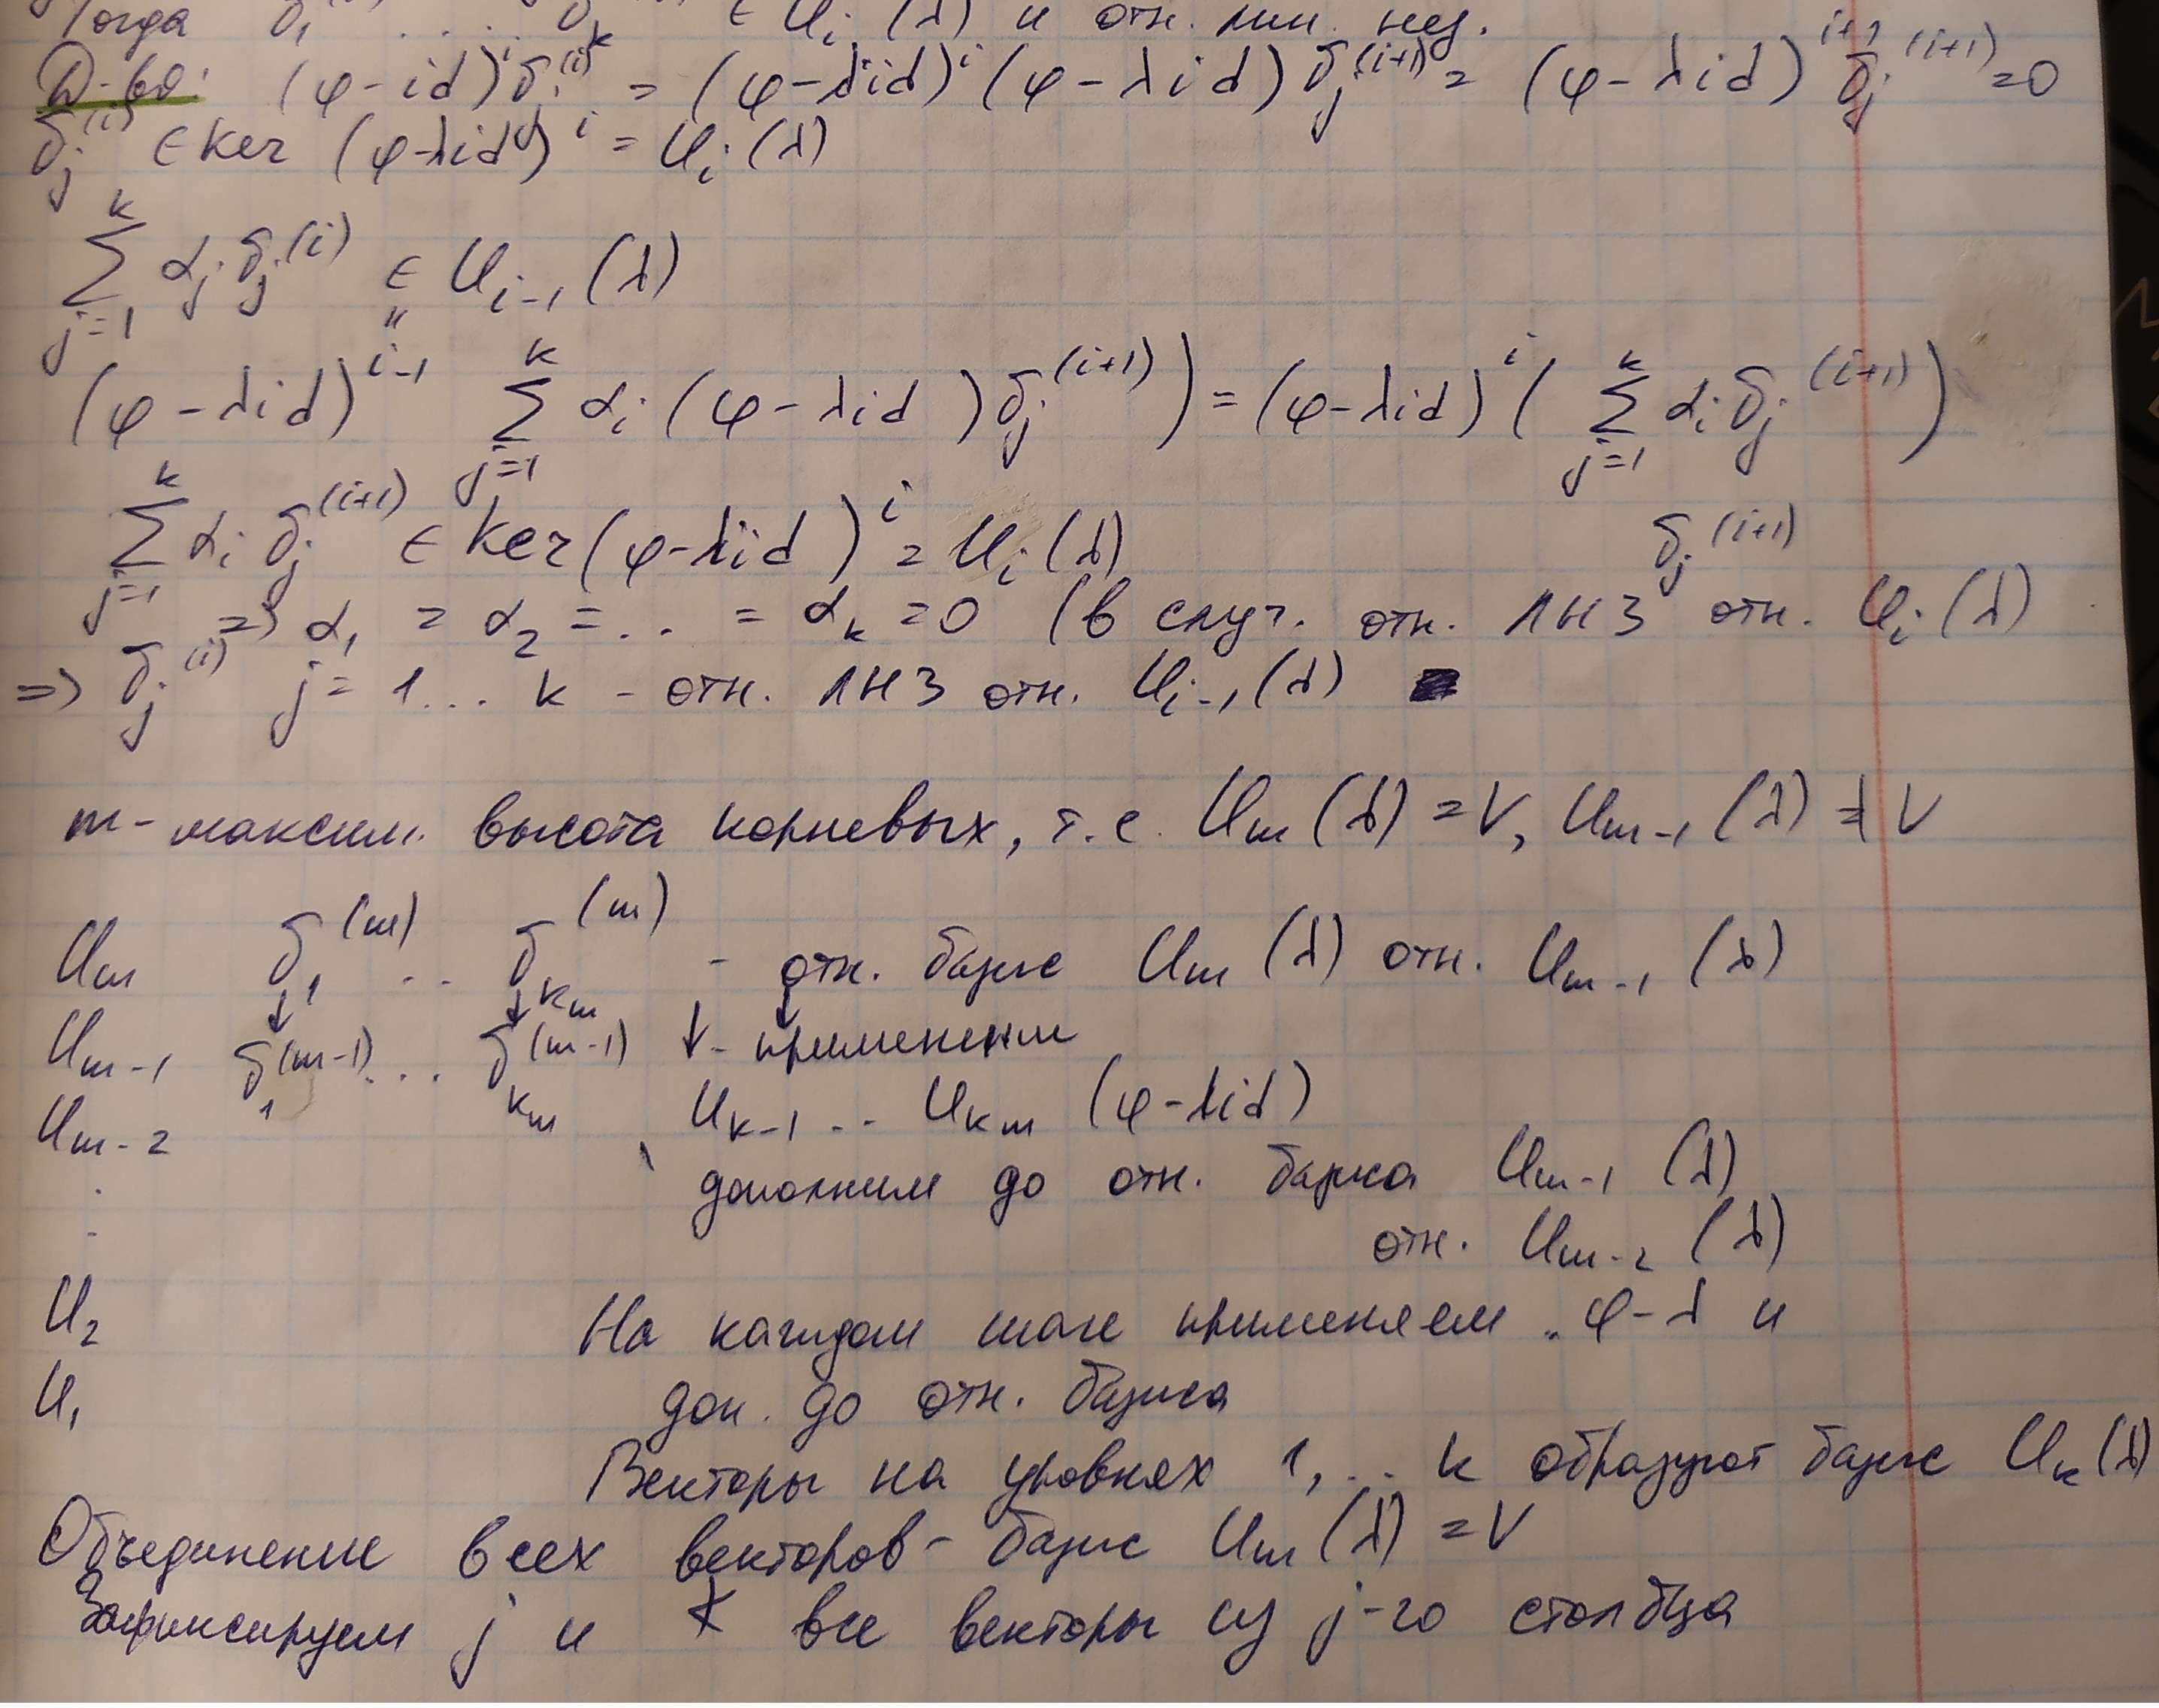
\includegraphics[width=10cm]{pics/l60_1}
            \centering
    \end{figure}

    \begin{figure}[H]
            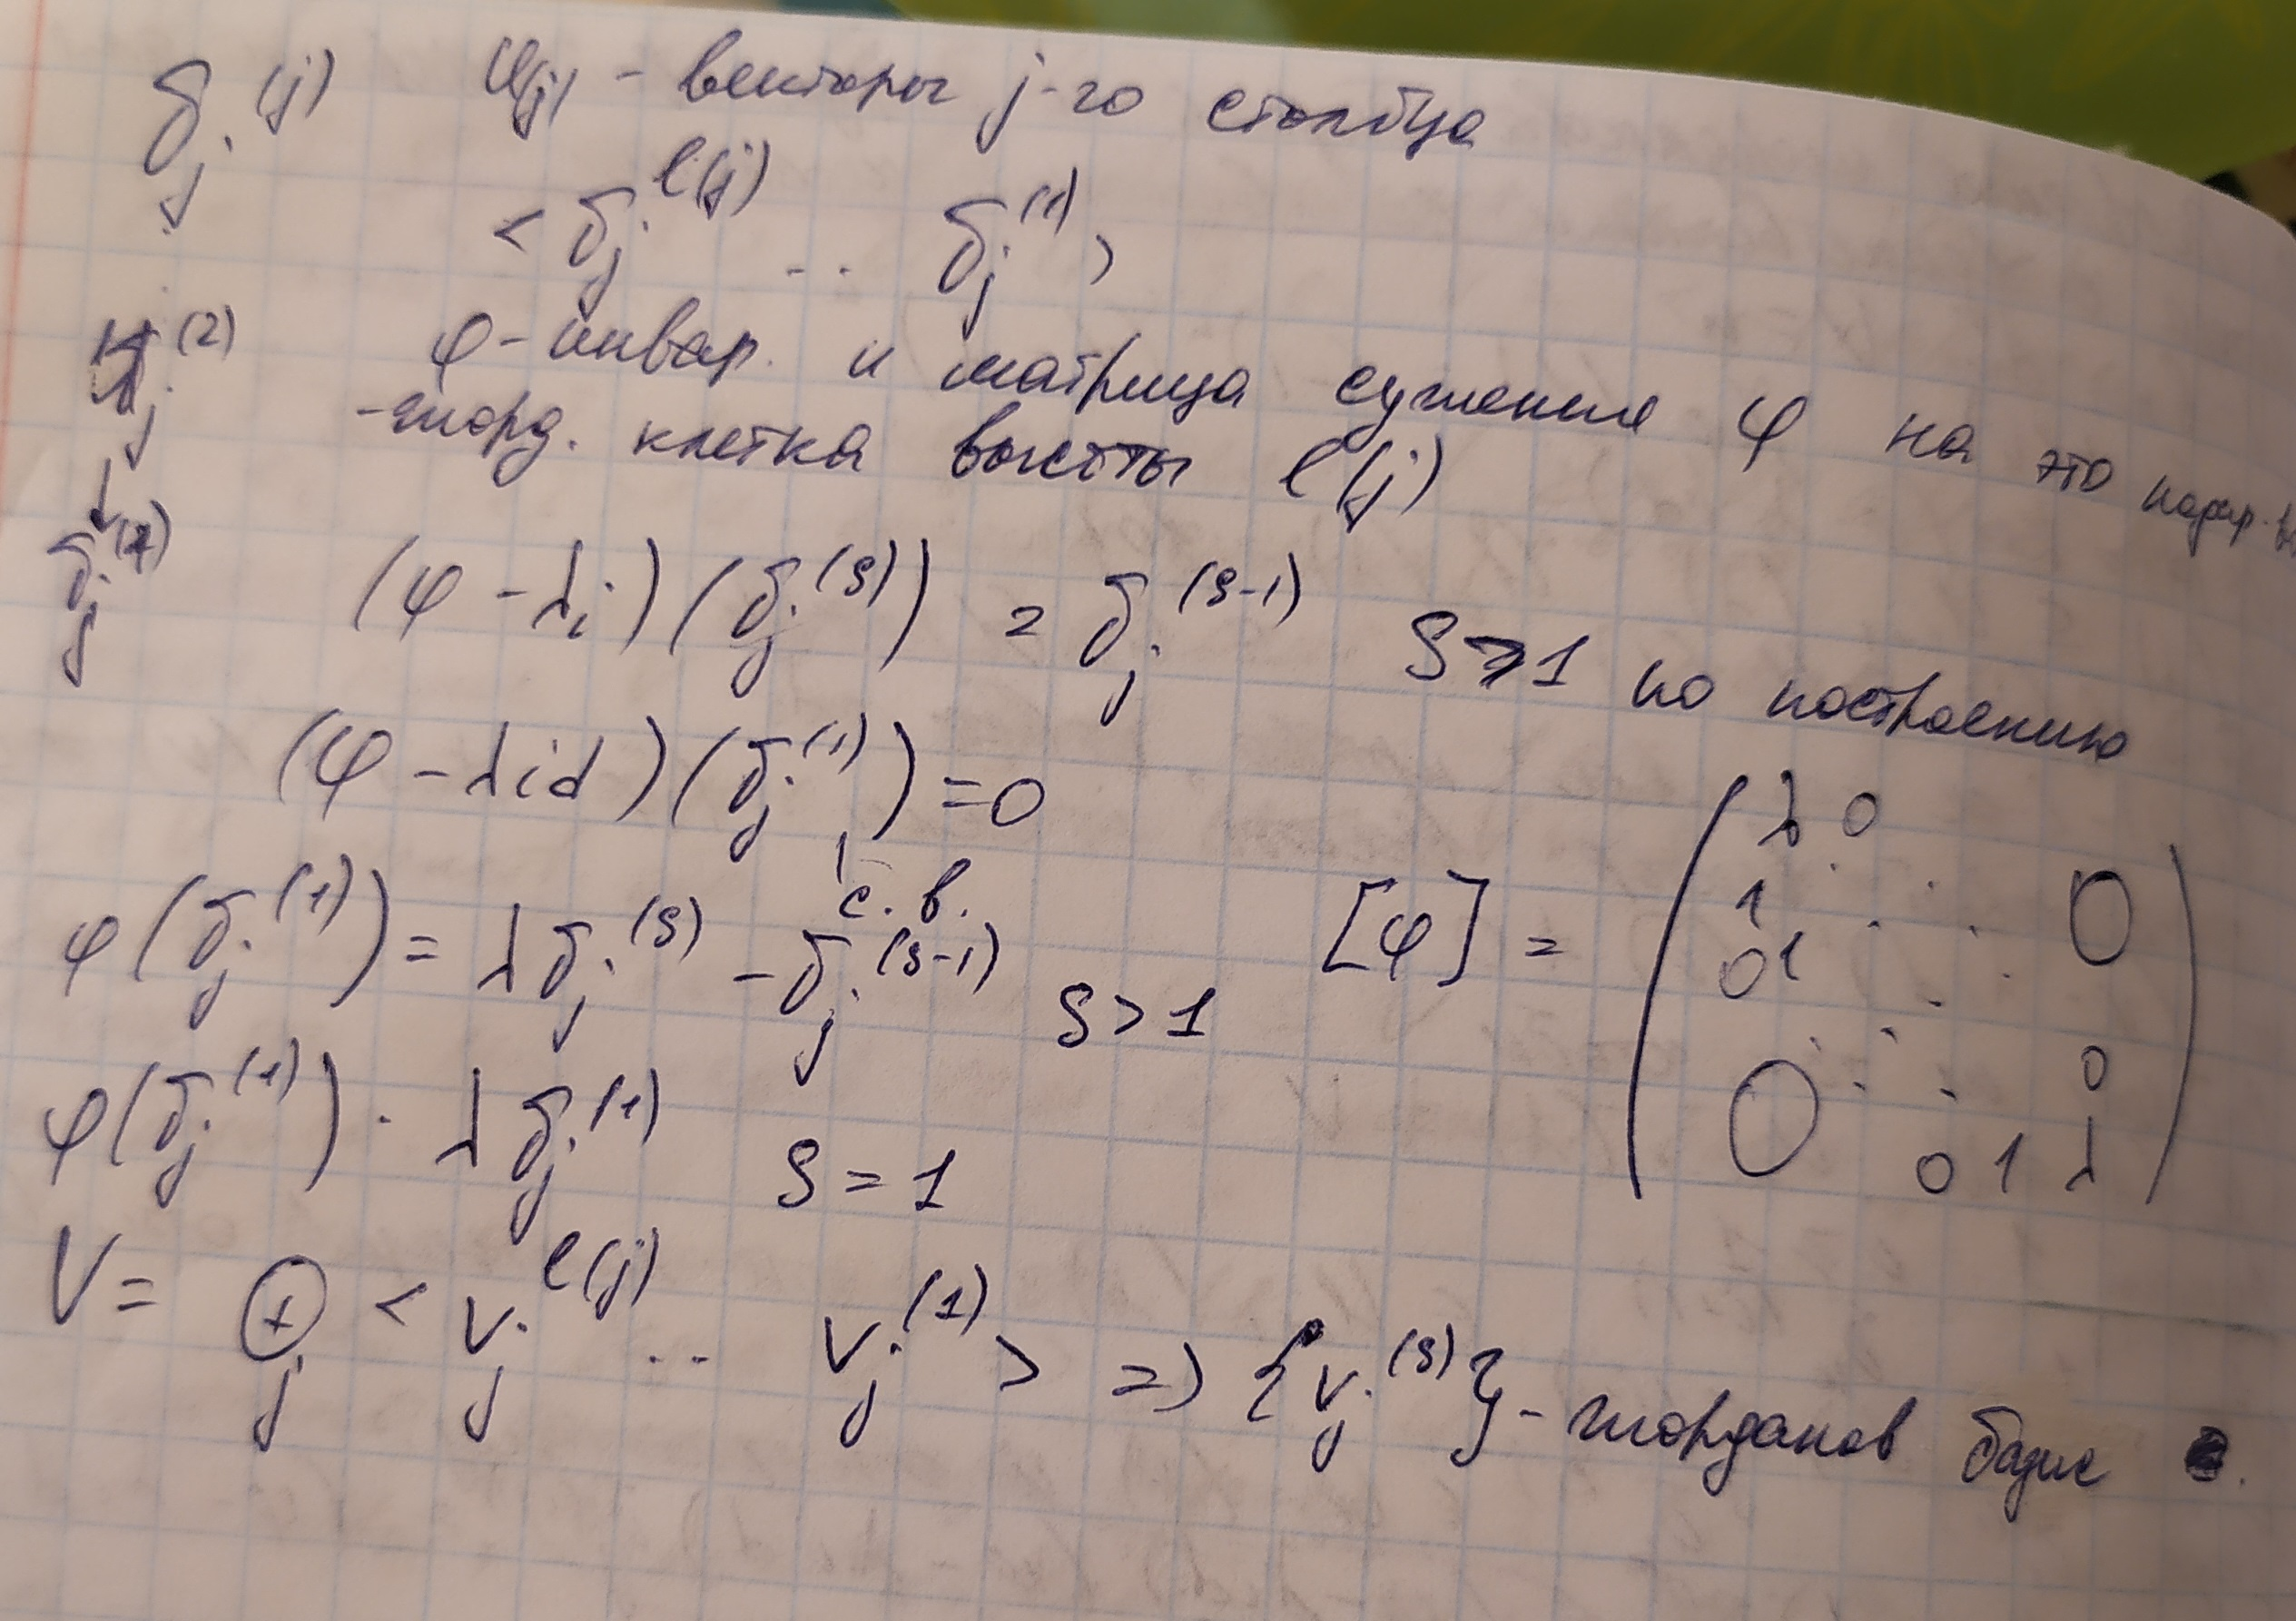
\includegraphics[width=10cm]{pics/l60_2}
            \centering
    \end{figure}

    \section{Единственность жордановой формы оператора.}

    *здесь когда-нибудь будет что-то*

    \begin{consequence}
      *здесь когда-нибудь будет следствие*
    \end{consequence}

    \begin{consequence}
      *здесь когда-нибудь будет следствие*
    \end{consequence}

    \begin{figure}[H]
            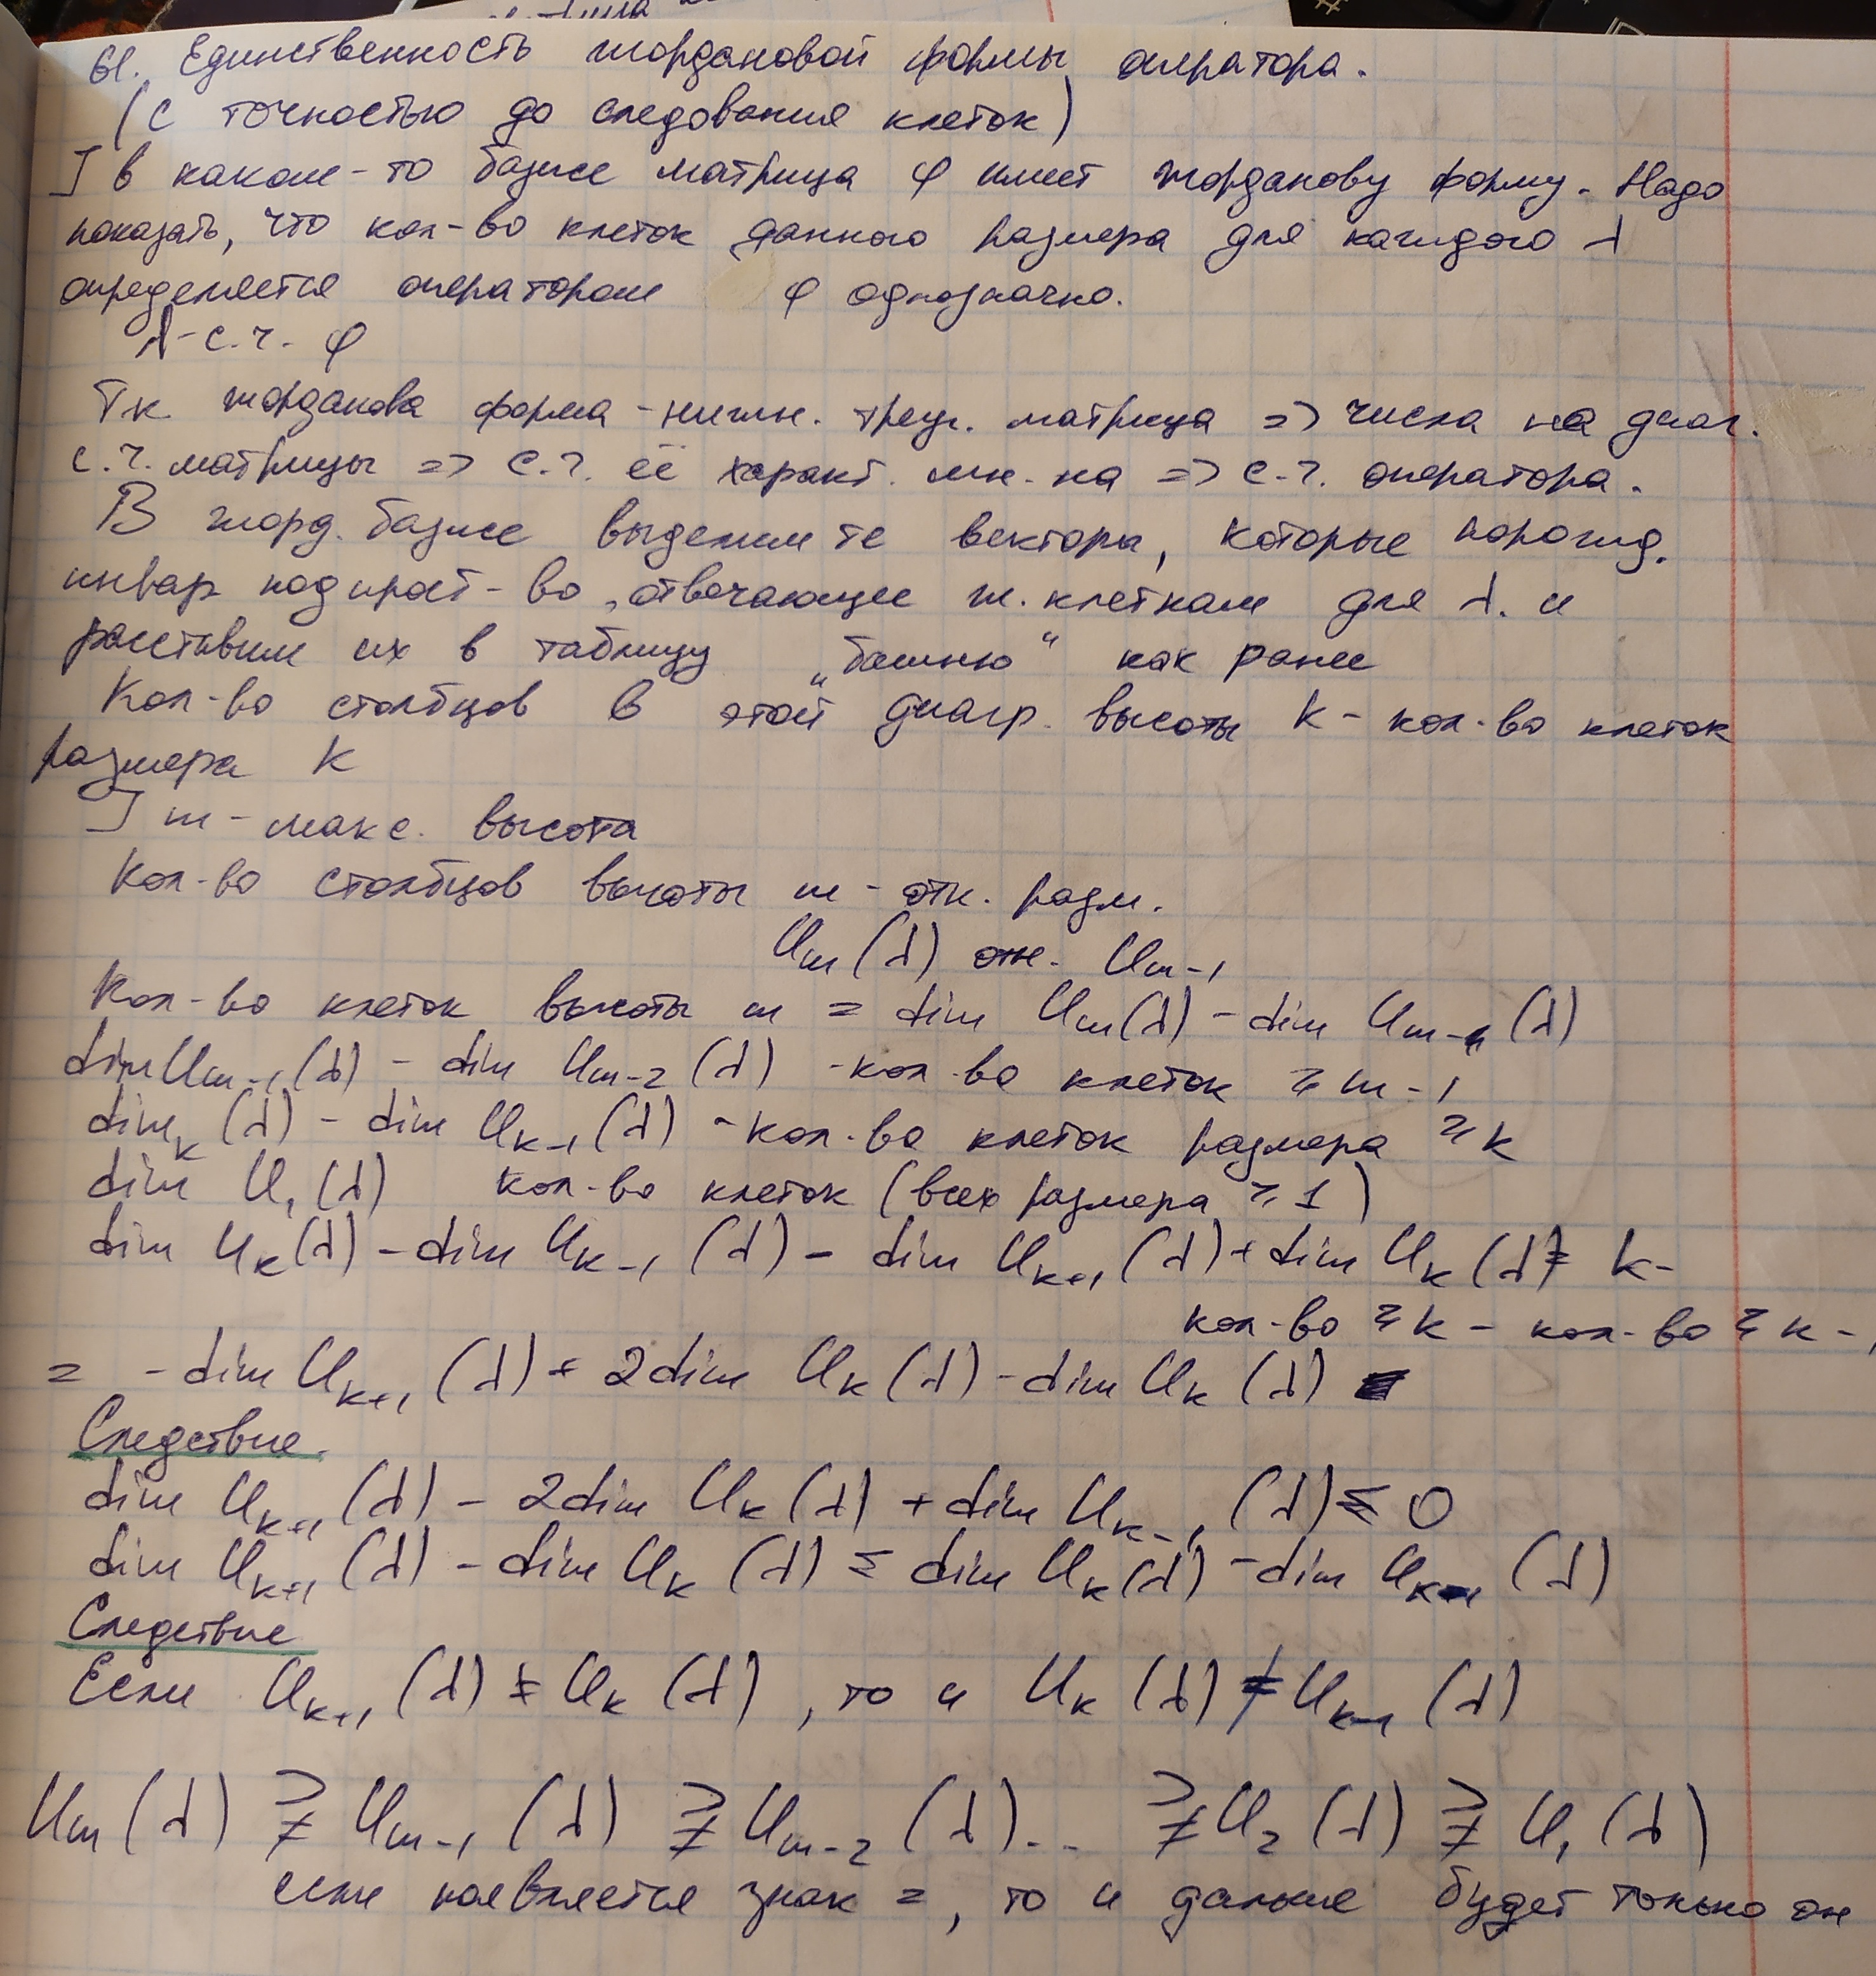
\includegraphics[width=10cm]{pics/l61}
            \centering
    \end{figure}
\end{document}
